\chapter{壓力、自由能與能量漲落}

\lectureoverview{我們不預設分子撞擊器壁的動力學圖像，而是從配分函數推導壓力。一個幾何引理將絕熱導數轉換為定溫導數，亥姆霍茲自由能則提供通往\(\log Z\)的橋梁；接著以此推導理想氣體定律，作為第一個應用。之後，我們再用同一個配分函數推導平衡能量漲落及其與熱容量的關係。}

\section{讓數學檢驗直覺}

熱力學有種奇特的名聲：微積分雖然初等，選擇對什麼求導、又要固定什麼，卻可能相當微妙。我們刻意把問題限定為計算理想氣體的壓力。然而，推導答案的方法也應足夠通用，能適用於熟悉的分子圖像不再可靠的系統。

動力學的說法很容易理解：分子撞擊器壁，使動量的法向分量反向。單位時間內傳遞的動量給出力，單位面積所受的力則是壓力。我們已知三維中每個分子的平均動能為
\begin{equation}
 \left\langle \frac{p^2}{2m}\right\rangle=\frac{3}{2}T
 \qquad (k_B=1).
 \label{eq:sm5-mean-kinetic-energy}
\end{equation}
若速度分布具有各向同性，就可以估算碰撞率、每次碰撞傳遞的動量，以及由此產生的壓力。

但器壁本身似乎會破壞各向同性。緊鄰邊界的分子，為什麼應該和深處的分子具有相同的速率與方向分布？在平衡態下，就此處所需的精度而言，兩者確實相同；但這個結論應該由統計力學推導出來，而不該把它當作直覺偷偷帶進計算。分子間的碰撞又讓動力學論證更難看清。無相互作用氣體之所以容易處理，正是因為它是格外簡單的系統。

物理學有時最穩妥的做法，是暫時放下圖像，順著數學推演。先找出要求的量，運用一般關係進行推導，等到熟悉的公式浮現。最後直覺再回來；這時，是數學在檢驗直覺，而不是反過來。熱力學的樂趣，就在於這種推演所揭示的出人意料的關係。

我們要找的是狀態方程式，
\begin{equation}
 P=P(T,V,N),
 \label{eq:sm5-equation-of-state-target}
\end{equation}
其中\(N\)是物質的量，\(T\)是溫度，\(V\)是體積。令人信服的推導，在粒子彼此作用時，或物質是液體、電漿、固體時，也應該仍然成立。只有在最後計算配分函數時，才會特別限定為理想氣體。

\section{熵與亥姆霍茲自由能}

先回顧稍後會用到的正則系綜公式。對於以\(i\)標記的微觀態，
\begin{equation}
 \begin{aligned}
 S&=-\sum_i p_i\log p_i,\\
 p_i&=\frac{e^{-\beta E_i}}{Z},\\
 Z&=\sum_i e^{-\beta E_i}.
 \end{aligned}
 \label{eq:sm5-canonical-definitions}
\end{equation}
機率的對數為
\begin{equation}
 \log p_i=-\beta E_i-\log Z.
 \label{eq:sm5-log-probability}
\end{equation}
代入熵的定義可得
\begin{align}
 S
 &=-\sum_i p_i\log p_i \notag\\
 &=\beta\sum_i p_iE_i+\log Z\sum_i p_i \notag\\
 &=\beta E+\log Z.
 \label{eq:sm5-entropy-log-z}
\end{align}
這裡的\(E=\sum_i p_iE_i\)是平均能量。

\begin{classroomqa}
\audiencequestion{為什麼第二項只得到\(\log Z\)，而不是態數乘上\(\log Z\)？}
\lecturerresponse{求和的係數是\(p_i\)，不是\(1\)。由歸一化條件可得\(\sum_i p_i=1\)。換句話說，分子\(\sum_i e^{-\beta E_i}=Z\)會和分母中的\(Z\)相消。這一步並沒有用到態數。
\lecturetimestamp{00:14:25--00:14:55}}
\end{classroomqa}

在本講大部分內容採用的能量單位下，
\(\beta=1/T\)。將\eqref{eq:sm5-entropy-log-z}乘上\(T\)並重新整理，可得
\begin{equation}
 E-TS=-T\log Z.
 \label{eq:sm5-helmholtz-identity}
\end{equation}
左邊這個組合經常出現，因此值得給它一個名稱：
\begin{equation}
 A\equiv E-TS,
 \qquad
 A=-T\log Z.
 \label{eq:sm5-helmholtz-definition}
\end{equation}
它就是亥姆霍茲自由能。此刻，名稱不如這個恆等式本身重要；稍後將壓力改寫成配分函數的導數時，我們會用到這個恆等式。

\begin{figure}[t]
\centering
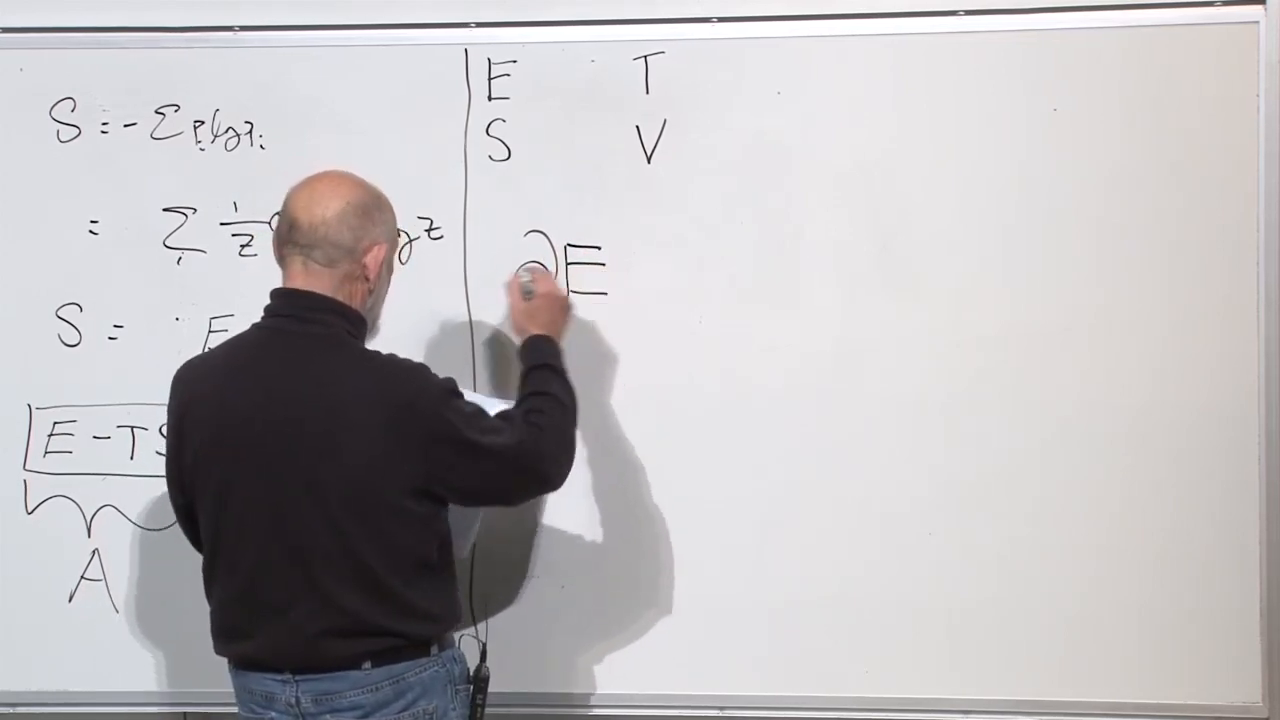
\includegraphics[width=0.90\textwidth]{lecture_05_figure_03.png}
\caption{將正則系綜的熵關係整理成
\(A=E-TS=-T\log Z\)。}
\lectureframe{00:16:50}
\end{figure}

\section{控制參數及其響應}

控制參數是實驗者能從外部改變的巨觀量。移動活塞可以改變體積，而不必操控個別分子。外加電場和磁場也是例子。在更一般的系綜中，粒子數也可以允許改變。

熱力學變數自然會成對出現，彼此互為共軛變數。在這個問題中，體積是控制參數，壓力則是它的響應。我們改變\(V\)；壓力則反映系統在能量上如何抵抗這項改變。稍後，能量的導數會明確說明這種配對關係。

\begin{classroomqa}
\audiencequestion{壓力本身可以視為控制參數嗎？}
\lecturerresponse{可以設計一種固定外部壓力的實驗；但在這裡採用的設定中，活塞位置決定體積，內部壓力則是響應量。壓力和體積互為共軛變數；控制哪一個，取決於所採用的系綜與裝置。
\lecturetimestamp{00:19:22--00:20:01}}
\end{classroomqa}

\begin{classroomqa}
\audiencequestion{這裡假設所有分子都相同嗎？還是這套論證只適用於氣體？}
\lecturerresponse{熱力學論證不需要這些限制。圓筒中可以有多種粒子、液體，甚至正在受壓的固體。一般壓力公式建立之後，理想氣體的配分函數才會作為一個特例出現。
\lecturetimestamp{00:20:02--00:20:39}}
\end{classroomqa}

\begin{classroomqa}
\audiencequestion{物質的量也可以透過另一種外部操作來改變嗎？}
\lecturerresponse{可以。粒子數也是一種可能的控制參數。若讓它動態改變，就會有相應的共軛變數，也就是化學勢。今晚的計算中，\(N\)維持不變。
\lecturetimestamp{00:20:39--00:20:57}}
\end{classroomqa}

\begin{classroomqa}
\audiencequestion{液態水和水蒸氣能同時處於平衡嗎？}
\lecturerresponse{可以，只要處於共存的溫度與壓力下。重力可能使液體位於蒸氣下方，但兩相仍可以具有相同溫度，並維持熱平衡。同一套一般性的統計力學架構也適用於此。
\lecturetimestamp{00:20:59--00:21:36}}
\end{classroomqa}

接下來的推導中，將能量和熵視為兩個獨立可調變數的函數：
\begin{equation}
 E=E(T,V),
 \qquad
 S=S(T,V).
 \label{eq:sm5-dependent-functions}
\end{equation}
溫度和體積是熱力學狀態空間的座標。能量和熵則為該空間中的每個平衡點指定數值。

\section{定熵導數}

我們最後需要的導數並不尋常：
\[
 \left(\frac{\partial E}{\partial V}\right)_S.
\]
雖然\(T\)和\(V\)是獨立座標，這個導數卻要求我們在改變\(V\)時，約束依賴函數\(S(T,V)\)維持不變。它是沿著\((T,V)\)平面中某條曲線的導數，而不是沿座標軸的導數。

\begin{classroomqa}
\audiencequestion{既然後面會用到導數\(dT/dV\)，\(T\)和\(V\)怎麼還能是獨立的？}
\lecturerresponse{在完整的狀態空間中，兩者是獨立的。施加約束\(S(T,V)=\mathrm{constant}\)後，允許的狀態便落在一維等值曲線上。沿著這條曲線，\(T\)成為\(V\)的函數，因此其斜率\(dT/dV\)有明確定義。
\lecturetimestamp{01:01:18--01:02:09}}
\end{classroomqa}

\begin{lemma}
如果\(E(T,V)\)和\(S(T,V)\)可微，則在\((\partial S/\partial T)_V\neq0\)成立的地方，
\begin{equation}
 \left(\frac{\partial E}{\partial V}\right)_S
 =
 \left(\frac{\partial E}{\partial V}\right)_T
 -
 \left(\frac{\partial E}{\partial S}\right)_V
 \left(\frac{\partial S}{\partial V}\right)_T.
 \label{eq:sm5-calculus-lemma}
\end{equation}
\end{lemma}

\begin{proof}
對於任意無窮小位移，
\begin{equation}
 dE=
 \left(\frac{\partial E}{\partial V}\right)_T dV
 +
 \left(\frac{\partial E}{\partial T}\right)_V dT.
 \label{eq:sm5-total-differential-e}
\end{equation}
在固定\(V\)時，可以依照鏈鎖律以\(S\)作為中間變數：
\begin{equation}
 \left(\frac{\partial E}{\partial T}\right)_V
 =
 \left(\frac{\partial E}{\partial S}\right)_V
 \left(\frac{\partial S}{\partial T}\right)_V.
 \label{eq:sm5-chain-rule-e-s-t}
\end{equation}

現在將位移限制在\(S\)維持不變的等值曲線上。沿著這條曲線，
\begin{equation}
 0=dS=
 \left(\frac{\partial S}{\partial V}\right)_T dV
 +
 \left(\frac{\partial S}{\partial T}\right)_V dT.
 \label{eq:sm5-constant-entropy-differential}
\end{equation}
解出曲線的斜率，可得
\begin{equation}
 \left(\frac{dT}{dV}\right)_S
 =
 -
 \frac{\left(\frac{\partial S}{\partial V}\right)_T}
 {\left(\frac{\partial S}{\partial T}\right)_V}.
 \label{eq:sm5-entropy-contour-slope}
\end{equation}
將\eqref{eq:sm5-total-differential-e}除以\(dV\)，利用
\eqref{eq:sm5-chain-rule-e-s-t}，再代入
\eqref{eq:sm5-entropy-contour-slope}：
\begin{align}
 \left(\frac{\partial E}{\partial V}\right)_S
 &=
 \left(\frac{\partial E}{\partial V}\right)_T
 +
 \left(\frac{\partial E}{\partial S}\right)_V
 \left(\frac{\partial S}{\partial T}\right)_V
 \left(\frac{dT}{dV}\right)_S \notag\\
 &=
 \left(\frac{\partial E}{\partial V}\right)_T
 -
 \left(\frac{\partial E}{\partial S}\right)_V
 \left(\frac{\partial S}{\partial V}\right)_T.
\end{align}
因子\((\partial S/\partial T)_V\)已經消去，證明得證。
\end{proof}

\begin{figure}[t]
\centering
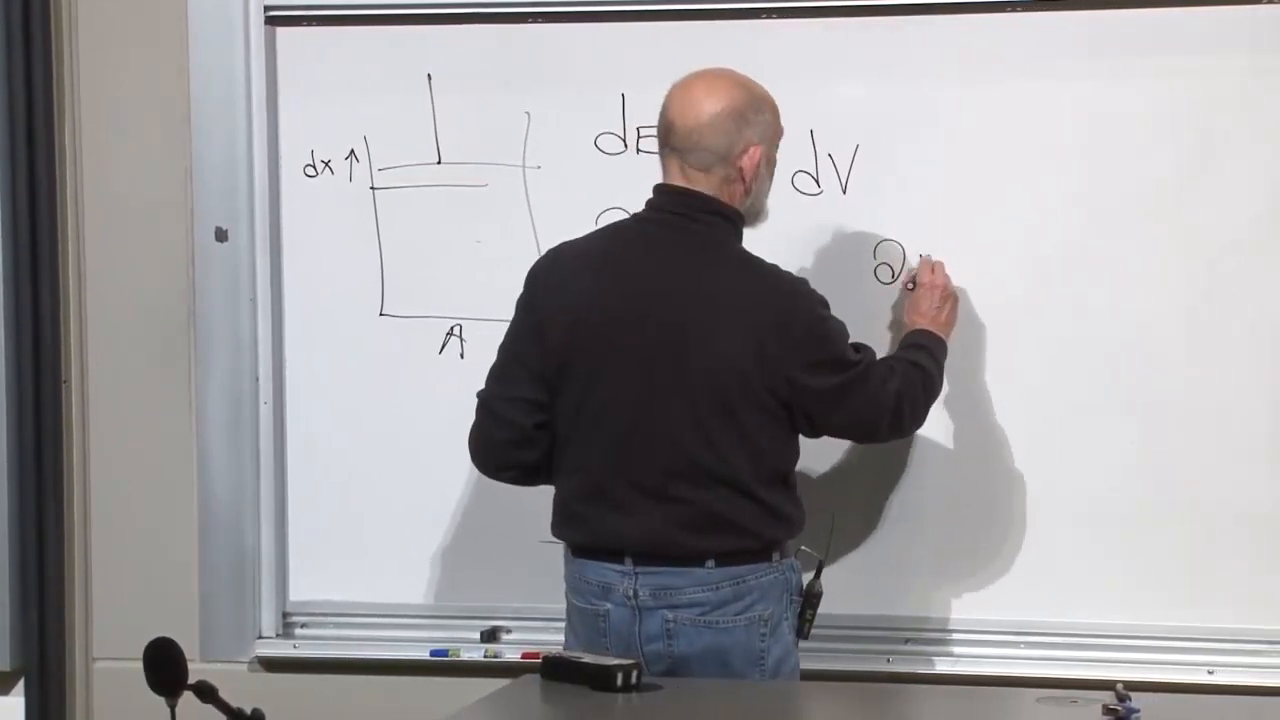
\includegraphics[width=0.90\textwidth]{lecture_05_figure_04.png}
\caption{定熵等值曲線上的計算，以及完成導數引理的消去步驟。}
\lectureframe{00:36:10}
\end{figure}

幾何圖像並非裝飾。它說明了為什麼看似奇特的固定\(S\)導數，可以用獨立座標\(T\)和\(V\)下的普通偏導數來計算。在推導中寫出\(\delta E/\delta V\)，也能提醒我們：這些符號代表沿指定路徑的小變化之比。

\begin{classroomqa}
\audiencequestion{\(dE\)的展開只是偏導數的一般定義嗎？}
\lecturerresponse{是的。全微分並沒有什麼特殊之處。唯一額外的步驟，是接著限制在等值曲線\(dS=0\)上；這會決定\(dT\)和\(dV\)之間的關係。
\lecturetimestamp{00:29:26--00:29:32}}
\end{classroomqa}

\begin{classroomqa}
\audiencequestion{消去時是否要求\((\partial S/\partial T)_V\)不為零？}
\lecturerresponse{是的。對一般的穩定系統，
\[
 \left(\frac{\partial S}{\partial T}\right)_V
 =\frac{C_V}{T}>0,
\]
因此可以合法地進行除法。特殊點則需要另外處理。哈密頓量固定時，提高溫度會使正則系綜的能量分布變寬，熵通常也會增加；降低溫度則會使分布變窄。這才是單調性論證在物理上正確的方向。
\lecturetimestamp{00:36:50--00:37:47}}
\end{classroomqa}

\section{活塞做功與絕熱條件}

現在為這個導數賦予物理意義。考慮一個截面積為\(\mathcal A\)的活塞。若活塞向外移動\(dx\)，則
\begin{equation}
 dV=\mathcal A\,dx.
 \label{eq:sm5-piston-volume}
\end{equation}
氣體對活塞施加\(P\mathcal A\)的力，因此氣體所做的功為
\begin{equation}
 \delta W_{\mathrm{by}}=P\mathcal A\,dx=P\,dV.
 \label{eq:sm5-piston-work}
\end{equation}
若沒有熱量進入氣體，能量守恆給出
\begin{equation}
 dE=-P\,dV.
 \label{eq:sm5-adiabatic-work}
\end{equation}
這個符號反映了實際的物理過程：膨脹時，氣體推升或加速活塞，而氣體本身的能量減少。

\begin{figure}[t]
\centering
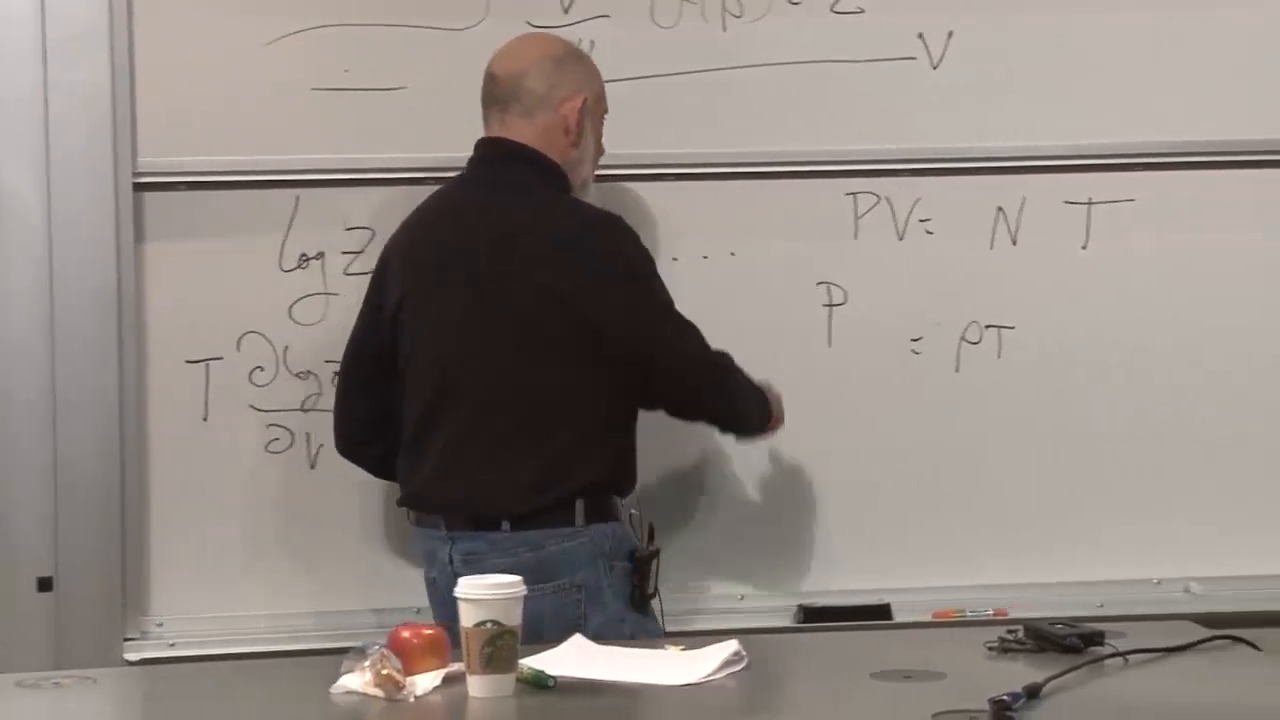
\includegraphics[width=0.90\textwidth]{lecture_05_figure_05.png}
\caption{活塞的幾何關係，以及推得的功的關係式\(dE=-P\,dV\)。}
\lectureframe{00:43:10}
\end{figure}

有兩項條件不可或缺。活塞必須移動得夠慢，讓系統始終任意接近平衡態；器壁也必須隔熱，避免能量以熱的形式進入。若拉動得很快，活塞可能在移動期間都沒有被任何分子撞到。快速壓縮則會產生衝擊波。這兩種過程都不能表示為一連串平衡態。

\emph{絕熱}一詞有時指沒有熱傳遞，有時指緩慢變化。在這裡所需的可逆過程中，兩項條件都要具備：變化是準靜態的，而且系統與外界隔熱。在這些條件下，過程也是等熵的。

\begin{classroomqa}
\audiencequestion{為什麼絕熱變化會使熵維持不變？}
\lecturerresponse{從量子力學的角度來看系統。系統的多體能階會隨體積改變。當\(V\)緩慢變化時，絕熱定理會使每個受佔據的能階連續地演變為相應的能階，而不在能階標籤之間發生躍遷。能量\(E_i(V)\)會改變，但佔據機率\(p_i\)維持不變。由於熵\(S=-\sum_i p_i\log p_i\)取決於這些機率，因此熵也維持不變。熱交換或不可逆運動則會使這個結論不再成立。
\lecturetimestamp{00:43:37--00:49:15}}
\end{classroomqa}

\begin{figure}[t]
\centering
\includegraphics[width=0.90\textwidth]{lecture_05_figure_06.png}
\caption{多體能階隨體積改變，而佔據機率仍對應於原來的能階標籤。}
\lectureframe{00:48:50}
\end{figure}

沿這條定熵路徑計算方程\eqref{eq:sm5-adiabatic-work}，即可辨認出壓力為
\begin{equation}
 P=-\left(\frac{\partial E}{\partial V}\right)_S.
 \label{eq:sm5-pressure-fixed-entropy}
\end{equation}
這就是壓力與體積之間的共軛關係。

\begin{classroomqa}
\audiencequestion{如果快速移動活塞，會發生什麼事？}
\lecturerresponse{系統會離開平衡態，此時具體的動力學過程便很重要。突然壓縮會產生衝擊波。在理想的自由膨脹中，活塞可以在分子撞上它之前就退開，因此不會做功；即使體積改變，能量仍保持不變。之後氣體會弛豫至熵增加的平衡態。這類過程無法用\eqref{eq:sm5-pressure-fixed-entropy}中的單一平衡態導數來描述。
\lecturetimestamp{00:58:30--01:01:15}}
\end{classroomqa}

\begin{classroomqa}
\audiencequestion{要用什麼定量條件判斷變化是否緩慢？}
\lecturerresponse{外部變化的時間尺度必須遠大於相關的內部弛豫時間。對氣體而言，在巨觀變化期間應該發生許多次分子碰撞和器壁碰撞。確切的時間尺度取決於物質和幾何形狀；準靜態極限本身則具有普遍性。
\lecturetimestamp{01:02:09--01:03:20}}
\end{classroomqa}

\section{從絕熱能量到配分函數}

物理關係式\eqref{eq:sm5-pressure-fixed-entropy}還不是容易計算的形式。正則系綜統計力學自然以溫度為變數，因為\(T\)直接出現在波茲曼因子中。微積分引理可以將不易處理的定熵導數，轉換成適合計算的形式：
\begin{align}
 P
 &=
 -\left(\frac{\partial E}{\partial V}\right)_T
 +
 \left(\frac{\partial E}{\partial S}\right)_V
 \left(\frac{\partial S}{\partial V}\right)_T.
 \label{eq:sm5-pressure-lemma-substitution}
\end{align}
定體積下，第一定律給出\(dE=T\,dS\)，因此
\begin{equation}
 \left(\frac{\partial E}{\partial S}\right)_V=T.
 \label{eq:sm5-e-s-temperature}
\end{equation}
於是
\begin{equation}
 P=
 -\left(\frac{\partial E}{\partial V}\right)_T
 +
 T\left(\frac{\partial S}{\partial V}\right)_T.
 \label{eq:sm5-pressure-fixed-temperature-pieces}
\end{equation}

\begin{classroomqa}
\audiencequestion{壓力公式中的負號從何而來？}
\lecturerresponse{負號源自氣體所做的功：在絕熱膨脹過程中，\(dE=-P\,dV\)。微積分引理的兩項之間本身就有一個負號；而\(P=-(\partial E/\partial V)_S\)中的整體負號會使兩項的符號都反轉，得到
\eqref{eq:sm5-pressure-fixed-temperature-pieces}。
\lecturetimestamp{00:52:40--00:53:14}}
\end{classroomqa}

兩個導數都在固定\(T\)的條件下計算，因此
\begin{align}
 P
 &=
 -\left(\frac{\partial}{\partial V}(E-TS)\right)_T \notag\\
 &=
 -\left(\frac{\partial A}{\partial V}\right)_T.
 \label{eq:sm5-pressure-free-energy}
\end{align}
最後代入\(A=-T\log Z\)：
\begin{equation}
 \boxed{
 P=
 T\left(\frac{\partial\log Z}{\partial V}\right)_T
 }.
 \label{eq:sm5-pressure-log-z}
\end{equation}

\begin{figure}[t]
\centering
\includegraphics[width=0.90\textwidth]{lecture_05_figure_07.png}
\caption{將推導整理為定溫下的形式：
\(P=-(\partial A/\partial V)_T
=T(\partial\log Z/\partial V)_T\)。}
\lectureframe{00:55:55}
\end{figure}

\eqref{eq:sm5-pressure-log-z}並未假設氣體是理想氣體。只要能算出交互作用流體、電漿或固體的配分函數，同一個導數就能給出其壓力。更一般地，每個外部控制參數都有一個共軛響應量，可藉由對適當的熱力學勢求導得到。配分函數包含了許多這類響應量：對\(\log Z\)關於\(\beta\)求導會得到能量，對體積求導則會得到壓力。

\section{理想氣體狀態方程式}

現在才限定為\(N\)個互不作用的粒子。保留經典相空間的歸一化因子，
\begin{equation}
 Z_N=
 \frac{1}{N!h^{3N}}
 \int d^{3N}q\,d^{3N}p\,
 \exp\!\left[
 -\beta\sum_{a=1}^{N}\frac{\mathbf p_a^2}{2m}
 \right].
 \label{eq:sm5-ideal-gas-partition-integral}
\end{equation}
其中有\(3N\)個位置座標和\(3N\)個動量座標。哈密頓量與位置無關，因此每個粒子都會貢獻一個容器體積因子：
\begin{equation}
 Z_N=
 \frac{V^N}{N!h^{3N}}I_p(\beta),
 \label{eq:sm5-ideal-gas-factorization}
\end{equation}
其中整個動量積分\(I_p(\beta)\)與\(V\)無關。

\begin{classroomqa}
\audiencequestion{為什麼位置積分和動量積分各有\(3N\)\(3N\)個？}
\lecturerresponse{每個\(N\)粒子都有三個空間座標和三個共軛動量分量。相空間的每一半各有\(3N\)個座標，而不是\(N\)個粒子再加上另外\(3N\)個粒子。
\lecturetimestamp{01:04:19--01:04:28}}
\end{classroomqa}

取對數後，體積的依賴關係就分離出來：
\begin{equation}
 \log Z_N
 =
 N\log V-\log N!-3N\log h+\log I_p(\beta).
 \label{eq:sm5-log-ideal-gas-partition}
\end{equation}
因子\(1/N!\)、\(h^{-3N}\)和\(I_p(\beta)\)都與體積無關。它們會影響絕對熵等其他問題，但不影響這裡要計算的導數。因此
\begin{equation}
 \left(\frac{\partial\log Z_N}{\partial V}\right)_T
 =\frac{N}{V}.
 \label{eq:sm5-log-z-volume-derivative}
\end{equation}
由方程\eqref{eq:sm5-pressure-log-z}可立即得到
\begin{equation}
 P=\frac{NT}{V},
 \qquad
 \boxed{PV=NT}.
 \label{eq:sm5-ideal-gas-law}
\end{equation}

\begin{classroomqa}
\audiencequestion{\(N\)還包含推導波茲曼分布時使用的複本嗎？}
\lecturerresponse{不包含。複本構造只是先前推導中用來計數的工具，這裡已不再使用。此處的\(N\)是這一份氣體樣本中的實際粒子數。
\lecturetimestamp{01:07:38--01:08:05}}
\end{classroomqa}

定義數密度
\begin{equation}
 \rho=\frac{N}{V}
 \label{eq:sm5-number-density}
\end{equation}
便可得到等價的形式
\begin{equation}
 P=\rho T.
 \label{eq:sm5-density-equation-of-state}
\end{equation}

\begin{classroomqa}
\audiencequestion{要得到密度形式，應該除以\(N\)還是\(V\)？}
\lecturerresponse{將\(PV=NT\)除以\(V\)：
\(P=(N/V)T=\rho T\)。這裡的\(\rho\)是數密度，不是質量密度。
\lecturetimestamp{01:08:45--01:09:16}}
\end{classroomqa}

\begin{figure}[t]
\centering
\includegraphics[width=0.90\textwidth]{lecture_05_figure_08.png}
\caption{\(\log Z\)對體積的導數，以及由此得到的理想氣體狀態方程式\(PV=NT\)，也就是\(P=\rho T\)。}
\lectureframe{01:09:25}
\end{figure}

改回實驗室使用的溫度\(T_K\)，
\begin{equation}
 PV=Nk_BT_K.
 \label{eq:sm5-ideal-gas-law-laboratory}
\end{equation}
這個熟悉的結果與動力學直覺一致，但如今它的推導所依據的架構，適用範圍遠超過自由氣體。

\section{另一個收穫：平衡漲落}

壓力的推導已經完成，但還有一個先前提出的問題尚未回答：配分函數還能提供什麼資訊？考慮一個與熱浴接觸的系統。它的能量並非固定不變，而是會進出系統；因此重複測量時，能量會在正則系綜的平均值附近漲落。

\begin{classroomqa}
\audiencequestion{現在可以計算先前提到的漲落了嗎？}
\lecturerresponse{可以。還有時間再說明一次相同的原理：\(Z\)的導數蘊含可測量的熱力學資訊。
\lecturetimestamp{01:10:37--01:10:50}}
\end{classroomqa}

\subsection{變異數與標準差}

對於隨機變數\(x\)，若\(\langle x\rangle=0\)，則可用\(\langle x^2\rangle\)衡量分布的寬度。對於一般分布，先將變數減去其平均值：
\begin{equation}
 \delta x=x-\langle x\rangle.
 \label{eq:sm5-centered-variable}
\end{equation}
所得變數的平均值為零：
\begin{equation}
 \langle\delta x\rangle
 =
 \langle x\rangle-\langle x\rangle=0,
 \label{eq:sm5-centered-mean}
\end{equation}
其均方為
\begin{align}
 (\Delta x)^2
 &\equiv
 \left\langle\left(x-\langle x\rangle\right)^2\right\rangle \notag\\
 &=
 \langle x^2\rangle
 -2\langle x\rangle^2
 +\langle x\rangle^2 \notag\\
 &=
 \langle x^2\rangle-\langle x\rangle^2.
 \label{eq:sm5-variance}
\end{align}
這就是變異數。變異數的正平方根\(\Delta x\)則是標準差。

\begin{classroomqa}
\audiencequestion{為什麼\(x-\langle x\rangle\)的平均值恰好等於零？}
\lecturerresponse{平均值具有線性，而\(\langle x\rangle\)本身已是數值。因此
\(\langle x-\langle x\rangle\rangle
=\langle x\rangle-\langle x\rangle=0\)。
\lecturetimestamp{01:14:02--01:14:22}}
\end{classroomqa}

\begin{classroomqa}
\audiencequestion{平方漲落、變異數、均方根寬度和標準差有什麼區別？}
\lecturerresponse{變異數是
\((\Delta x)^2=\langle x^2\rangle-\langle x\rangle^2\)。
標準差是變異數的平方根，即\(\Delta x\)。對於平均值為零的變數，標準差也等於其均方根值。
\lecturetimestamp{01:16:39--01:18:38}}
\end{classroomqa}

\begin{figure}[t]
\centering
\includegraphics[width=0.90\textwidth]{lecture_05_figure_09.png}
\caption{平移後的變數，以及推得\((\Delta x)^2=\langle x^2\rangle-\langle x\rangle^2\)的展開式。}
\lectureframe{01:17:20}
\end{figure}

\subsection{由配分函數求得能量矩}

對於正則系綜，
\begin{align}
 \langle E\rangle
 &=
 \frac{1}{Z}\sum_i E_i e^{-\beta E_i} \notag\\
 &=
 -\frac{1}{Z}\frac{\partial Z}{\partial\beta}
 =
 -\frac{\partial\log Z}{\partial\beta}.
 \label{eq:sm5-mean-energy-from-z}
\end{align}
乘上一個\(E_i\)因子，相當於對\(\beta\)求一次負導數。再求一次導數，就會得到\(E_i^2\)：
\begin{equation}
 \langle E^2\rangle
 =
 \frac{1}{Z}\sum_i E_i^2e^{-\beta E_i}
 =
 \frac{1}{Z}\frac{\partial^2 Z}{\partial\beta^2}.
 \label{eq:sm5-second-energy-moment}
\end{equation}
因此，能量的變異數為
\begin{align}
 (\Delta E)^2
 &=
 \langle E^2\rangle-\langle E\rangle^2 \notag\\
 &=
 \frac{1}{Z}\frac{\partial^2Z}{\partial\beta^2}
 -
 \frac{1}{Z^2}
 \left(\frac{\partial Z}{\partial\beta}\right)^2 \notag\\
 &=
 \frac{\partial^2\log Z}{\partial\beta^2}
 =
 -\frac{\partial\langle E\rangle}{\partial\beta}.
 \label{eq:sm5-energy-variance-beta}
\end{align}
再次可見，看似複雜的可觀測量其實可以寫成\(\log Z\)的導數。

\begin{figure}[t]
\centering
\includegraphics[width=0.90\textwidth]{lecture_05_figure_10.png}
\caption{將\(\beta\)的二階導數\(\log Z\)與能量變異數連結起來。}
\lectureframe{01:29:00}
\end{figure}

\subsection{熱容量與漲落的大小}

以本講採用的單位表示，\(T=1/\beta\)，因此
\begin{equation}
 -\frac{\partial}{\partial\beta}
 =
 T^2\frac{\partial}{\partial T}.
 \label{eq:sm5-beta-temperature-derivative}
\end{equation}
定義整個樣本在定體積下的熱容量為
\begin{equation}
 C_V\equiv
 \left(\frac{\partial\langle E\rangle}{\partial T}\right)_V.
 \label{eq:sm5-heat-capacity}
\end{equation}
方程\eqref{eq:sm5-energy-variance-beta}便成為
\begin{equation}
 \boxed{(\Delta E)^2=T^2C_V}
 \qquad (k_B=1).
 \label{eq:sm5-energy-fluctuation-lecture-units}
\end{equation}
若改用實驗室溫度\(T_K\)，其中
\(\beta=(k_BT_K)^{-1}\)，則有
\begin{equation}
 \boxed{(\Delta E)^2=k_BT_K^2C_V}.
 \label{eq:sm5-energy-fluctuation-laboratory}
\end{equation}

\begin{figure}[t]
\centering
\includegraphics[width=0.90\textwidth]{lecture_05_figure_11.png}
\caption{從\(\beta\)導數轉換為定容熱容量，並恢復\(k_B\)因子。}
\lectureframe{01:31:10}
\end{figure}

\begin{classroomqa}
\audiencequestion{導數必須指定在定體積下，而不是定壓下嗎？}
\lecturerresponse{是的。這個正則系綜的推導會固定哈密頓量的外部控制參數，包括\(V\)。因此得到的量是\(C_V\)。定壓系綜允許體積和功發生漲落，並且需要使用相應的熱力學勢；不能只在\eqref{eq:sm5-energy-fluctuation-laboratory}中把\(C_V\)換成\(C_P\)。
\lecturetimestamp{01:29:01--01:29:28; 01:32:50--01:33:21}}
\end{classroomqa}

\begin{classroomqa}
\audiencequestion{\(C_V\)是材料常數嗎？}
\lecturerresponse{一般而言不是。它可能隨溫度、體積、相態和組成而變。此外，這裡的\(C_V\)是整個樣本的熱容量，屬於廣延量。只有再除以質量、粒子數或物質的量，才會得到比熱或莫耳熱容量。
\lecturetimestamp{01:31:47--01:32:21; 01:33:23--01:34:55}}
\end{classroomqa}

對一般的廣延物質，\(C_V\)與\(N\)成正比，因此\((\Delta E)^2\)與\(N\)成正比，而\(\Delta E\)與\(\sqrt{N}\)成正比。平均能量本身則與\(N\)成正比。因此
\begin{equation}
 \frac{\Delta E}{\langle E\rangle}\sim\frac{1}{\sqrt{N}}.
 \label{eq:sm5-relative-fluctuation-scaling}
\end{equation}
巨觀系統的相對漲落非常小，微觀樣本則能直接呈現這些漲落。\(k_B\)出現在\eqref{eq:sm5-energy-fluctuation-laboratory}中，顯示熱力學可觀測量與分子的離散性相連；換句話說，它也連結了巨觀單位與阿伏加德羅數量級的計數。

壓力與漲落如今都從同一個量導出：
\[
 P=T\left(\frac{\partial\log Z}{\partial V}\right)_T,
 \qquad
 (\Delta E)^2=\frac{\partial^2\log Z}{\partial\beta^2}.
\]
這是本講的核心要點。辨明正確的約束條件後，配分函數便不只是用來將機率歸一化；它的導數也系統地整理出可測量的熱力學性質。